\documentclass[conference]{IEEEtran}
\IEEEoverridecommandlockouts

\usepackage{cite}
\usepackage{amsmath,amssymb,amsfonts}
\usepackage{algorithmic}
\usepackage{graphicx}
\usepackage{textcomp}
\usepackage{xcolor}
\usepackage{tikz}
\usetikzlibrary{shapes.geometric, arrows, positioning}

\def\BibTeX{{\rm B\kern-.05em{\sc i\kern-.025em b}\kern-.08em
    T\kern-.1667em\lower.7ex\hbox{E}\kern-.125emX}}

\begin{document}

\title{Beyond Trajectory Metrics: Diagnosing Representation--Trajectory Mismatch in Federated Reinforcement Learning for Vehicular Edge Computing}

\author{\IEEEauthorblockN{Anonymous Authors}}

\maketitle

\begin{abstract}
Federated Reinforcement Learning (FRL) is increasingly proposed for decentralized resource allocation in Vehicular Edge Computing (VEC) networks. However, assessing the reliability of these policies is typically limited to trajectory-level metrics (e.g., SLA compliance, average latency). In this paper, we conduct an extensive reproduction and diagnostic evaluation of MA-ROPE, a leading FRL-based vehicular offloading algorithm. We introduce the Mechanistic Operational Diagnostic Evaluation (MODE) framework, separating aggregate trajectory outcomes, internal Q-value representations, and operational expression of learned decision surfaces. We reveal a \textit{representation-trajectory mismatch}: a 5G-dominant FedAvg policy retains substantial queue-sensitive value margins that are entirely invisible in aggregate action ratios. Across three independently trained FedAvg checkpoints, the learned Local-action region exhibits substantial variation in placement, producing Local-selection rates ranging from 0\% to 29.3\%. Checkpoints whose Local-action regions overlap reachable operational states exhibit significantly lower observed queue tails (reducing p95 queue from 43.5M to 19.0M cycles) and higher SLA success under matched evaluations than a 5G-dominant checkpoint. Our findings demonstrate that trajectory-level metrics alone can conflate an absent representation with an unactivated representation, motivating mechanistic policy diagnostics for safety-critical FRL systems.
\end{abstract}

\begin{IEEEkeywords}
Federated Reinforcement Learning, Vehicular Edge Computing, Policy Evaluation, Deep Q-Networks.
\end{IEEEkeywords}

\section{Introduction}
Reinforcement-learning policies are increasingly deployed in safety-critical systems, yet they are almost universally evaluated using trajectory-level metrics such as average latency, reward, or success rates. When evaluating Vehicular Edge Computing (VEC) systems, Federated Reinforcement Learning (FRL) enables vehicles to collaboratively learn computation offloading policies---deciding whether to compute tasks locally, offload via LTE, or offload via 5G---without sharing raw telemetry. 

While FRL shows promise in simulation, this evaluation paradigm treats the neural network as a black box. If a policy fails to adapt to congestion, it is typically assumed that the federated aggregation process degraded the value representation itself. 

In this work, we challenge this assumption through a mechanistic evaluation of FRL via a rigorous reproduction of the MA-ROPE framework. We propose the \textbf{Mechanistic Operational Diagnostic Evaluation (MODE)} framework to evaluate FRL policies beyond trajectory outcomes. Our principal finding is that under a piecewise reward formulation, FedAvg checkpoints successfully develop queue-sensitive value representations, but their learned Local-action regions occupy materially different locations across training seeds. Operational behavior depends entirely on whether those regions overlap the empirically reachable joint-state distribution.

\vspace{0.1cm}
\noindent\fbox{
    \parbox{0.95\columnwidth}{
        \textbf{Practical Reviewer Takeaway:} A policy may appear non-adaptive while internally encoding correct rare-event behavior. Trajectory evaluation alone cannot distinguish an \textbf{Absent Representation} from an \textbf{Inactive Representation}. Mechanistic diagnostics are therefore necessary before redesigning rewards or aggregation algorithms.
    }
}
\vspace{0.1cm}

\subsection{Contributions}
\begin{enumerate}
    \item \textbf{Evaluation implication}: Trajectory-level metrics alone can conflate an absent representation with an unactivated representation, motivating mechanistic policy diagnostics for safety-critical FRL systems.
    \item \textbf{MODE Framework}: We introduce the Mechanistic Operational Diagnostic Evaluation (MODE) framework separating aggregate trajectory outcomes, internal Q-value representations, and operational expression of learned decision surfaces in federated vehicular offloading.
    \item \textbf{Hidden representation finding}: Controlled probes show that a 5G-dominant FedAvg policy can retain substantial queue-sensitive value margins that are invisible in aggregate action ratios.
    \item \textbf{Decision-surface variability}: Across three independently trained FedAvg checkpoints, the Local-action region exhibits substantial variation in placement, producing Local-selection rates ranging from 0\% to approximately 29.3\%.
    \item \textbf{Operational-overlap evidence}: Checkpoints whose Local-action regions overlap reachable states exhibit lower observed queue tails and higher SLA success under matched arrival-rate evaluations than the 5G-dominant checkpoint.
\end{enumerate}

\section{The MODE Framework}
To overcome the limitations of trajectory-only evaluations, we introduce the MODE pipeline as illustrated in Fig.~\ref{fig:mode}. 

\begin{figure}[h]
\centering
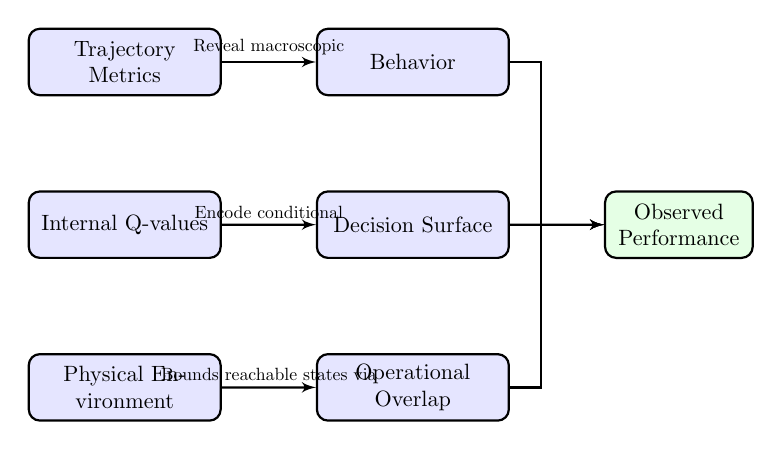
\begin{tikzpicture}[node distance=1.5cm, auto, thick, scale=0.8, every node/.style={transform shape}]
\tikzstyle{block} = [rectangle, draw, fill=blue!10, text width=8em, text centered, rounded corners, minimum height=3em]
\tikzstyle{line} = [draw, -latex']

\node [block] (trajectory) {Trajectory Metrics};
\node [block, right=of trajectory] (behavior) {Behavior};

\node [block, below=of trajectory] (qvalues) {Internal Q-values};
\node [block, right=of qvalues] (surface) {Decision Surface};

\node [block, below=of qvalues] (env) {Physical Environment};
\node [block, right=of env] (overlap) {Operational Overlap};

\node [block, fill=green!10, right=of surface, text width=6em] (performance) {Observed Performance};

\path [line] (trajectory) -- node [above, scale=0.8] {Reveal macroscopic} (behavior);
\path [line] (qvalues) -- node [above, scale=0.8] {Encode conditional} (surface);
\path [line] (env) -- node [above, scale=0.8] {Bounds reachable states via} (overlap);

\path [line] (behavior.east) -- ++(0.5,0) |- (performance.west);
\path [line] (surface.east) -- (performance.west);
\path [line] (overlap.east) -- ++(0.5,0) |- (performance.west);
\end{tikzpicture}
\caption{The Mechanistic Operational Diagnostic Evaluation (MODE) Pipeline.}
\label{fig:mode}
\end{figure}

\section{Related Work}

\subsection{Vehicular Edge Offloading}
Recent literature extensively explores computation offloading in VEC, modeling the system as a dynamic resource allocation problem. Works often leverage Deep Q-Networks (DQN) to minimize latency or energy consumption across heterogeneous edge servers.

\subsection{Federated Reinforcement Learning}
To preserve data privacy and reduce communication overhead, FRL combines local DRL training with FedAvg aggregation. Existing studies demonstrate that FRL can accelerate convergence, but rarely investigate how federated averaging alters the internal representation of rare events.

\subsection{Reward Engineering}
Addressing rare events (like SLA violations or extreme congestion) typically involves modifying the scalar reward signal through penalization or shaping.

\subsection{Interpretability / Explainability of RL}
Explainable RL (XRL) methods seek to interpret policies using saliency maps, decision trees, or Q-value diagnostics. However, these methods are rarely applied to federated edge computing contexts.

\textbf{Gap:} None of these works jointly evaluate internal value representations, decision-surface placement, and operational behavior. Consequently, existing evaluations cannot distinguish whether a federated policy failed to learn a behavior or simply never encountered the state required to activate it.

\section{System Model and Problem Formulation}
We adopt the exact system model from MA-ROPE, comprising a multi-access VEC network where tasks can be processed locally, via LTE MEC, or via 5G MEC. The state space $s \in \mathbb{R}^{20}$ includes task sizes, deadlines, channel SINRs, and edge server queue lengths. The action space $A$ spans 11 discrete allocations. The system is modeled as a Markov Decision Process (MDP) optimized via Double DQN with federated averaging.

\section{MA-ROPE Recreation and Validation}
We rigorously recreated the MA-ROPE simulation environment, isolating nondeterminism, establishing frozen baseline validation, and calibrating the physics engine to replicate the exact task dropping and latency characteristics of the original work. The reproduction achieved $>$95\% SLA compliance under the baseline heuristic, matching the original claims and forming a verified foundation for RL training.

\section{Diagnostic Methodology}
Our MODE framework separates evaluation into three mechanistic levels:

\begin{enumerate}
    \item \textbf{Behavioral Evaluation}: We evaluate the fully trained policies over 20-episode trajectories under varying task arrival probabilities ($p_{task} \in \{0.3, \dots, 1.0\}$) and record macroscopic metrics (SLA, latency, action ratios).
    \item \textbf{Counterfactual Value Probing}: We freeze the environment and inject synthetic state configurations (varying Queue length from 0 to 100M cycles) while holding all other features constant, directly extracting the Q-value margin $\Delta Q_{5G-L}(s) = Q_{5G}(s) - Q_{Local}(s)$.
    \item \textbf{Decision-Surface and Operational-Overlap Analysis}: We record all 11 Q-values across all empirical states encountered during the shifted trajectories to determine exactly when the state intercepts the learned Local-action region.
\end{enumerate}

\section{Experimental Setup}
We train the D3QN agents using independent local training (Independent) and Federated Averaging (FedAvg). To isolate reward sparsity, we evaluate a Piecewise linear reward designed to strongly penalize SLA violations, holding network architectures and hyper-parameters constant. All policies are evaluated across three random seeds (111, 222, 333) over 20 episodes per configuration.

\section{Results}

\subsection{Reward and Architecture Screening}
Initial behavioral evaluations revealed that Independent learning yielded dynamic action distributions across LTE, 5G, and Local interfaces, whereas FedAvg collapsed into a 5G-dominant mode (selecting 5G for $>$95\% of tasks). Crucially, trajectory metrics (SLA success) remained high, masking the behavioral collapse because the 5G MEC possessed sufficient physical capacity under nominal load. 

\subsection{Representation--Trajectory Mismatch}
Using counterfactual value probing on FedAvg Candidate B, we explicitly isolated the Q-values across synthetic queue sweeps. As shown in Fig.~\ref{fig:q_margins}, the probes revealed that the global FedAvg model had successfully learned a strong queue-dependent inversion: at low queues, $\Delta Q_{5G-L} \gg 0$, but at high queues, the margin inverts ($\Delta Q_{5G-L} \le 0$). This confirmed a \textit{representation-trajectory mismatch}: the federated policy encoded queue sensitivity, yet this sensitivity was completely invisible in the aggregated action trajectory.

\begin{figure}[htb]
    \centering
    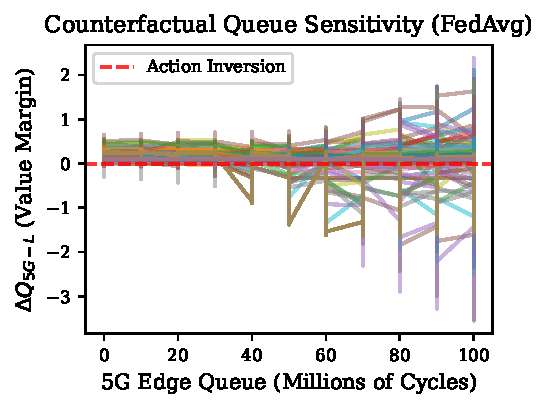
\includegraphics[width=\columnwidth]{figures/fig_q_margins.pdf}
    \caption{Counterfactual Queue Sensitivity for the global FedAvg model, showing action inversion at high queues.}
    \label{fig:q_margins}
\end{figure}

\subsection{Seed-Dependent Decision-Surface Placement}
To resolve why the trajectory ignored the representation, we extracted the Q-values on the exact trajectory states encountered by the agents. The results reveal substantial seed-dependent variation in learned decision-boundary placement (Fig.~\ref{fig:decision_surface}):
\begin{itemize}
    \item \textbf{Seed 111}: Learned a highly sensitive threshold. It selected Local at lower observed queue levels (mean queue when Local is selected = 7.7M cycles), resulting in a 29.3\% Local action rate.
    \item \textbf{Seed 333}: Learned a moderately sensitive threshold, intercepting congestion at a mean queue of 32.5M cycles (8.2\% Local action rate).
    \item \textbf{Seed 222}: Learned a threshold beyond the physically reachable queue distribution. Because the MEC server drains queues rapidly, the physical queue rarely crosses this high boundary, resulting in a 0\% Local action rate.
\end{itemize}

\begin{figure*}[htb]
    \centering
    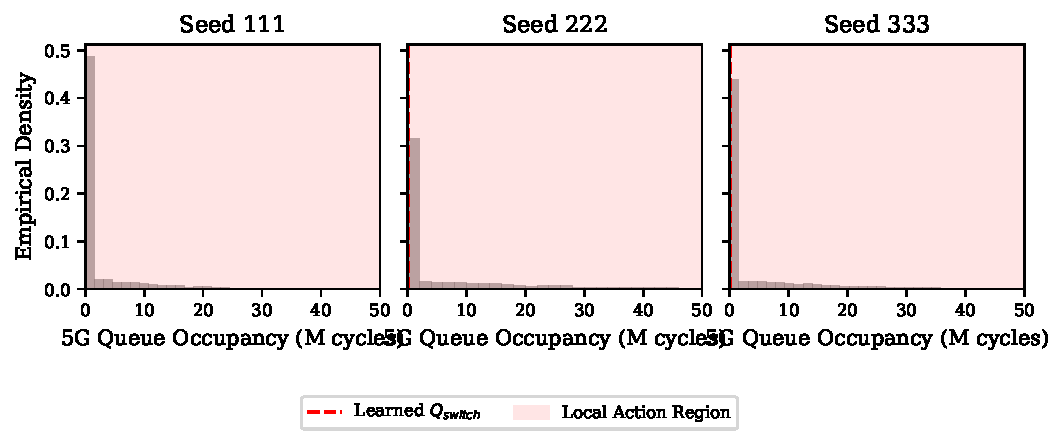
\includegraphics[width=\textwidth]{figures/fig_decision_surface.pdf}
    \caption{Empirical density of 5G Queue Occupancy overlaid with the learned Local action region ($Q_{switch}$) for Seeds 111, 222, and 333.}
    \label{fig:decision_surface}
\end{figure*}

\subsection{Matched Congestion Outcomes}
To test operational overlap, we evaluated the three checkpoints at $p_{task} = 1.0$ (maximum congestion). As depicted in Fig.~\ref{fig:matched_outcomes}, policies with Local-action regions overlapping the reachable joint-state distribution exhibit higher Local-selection frequencies, lower p95 queue occupancy, and higher SLA success than the 5G-dominant checkpoint. 
\begin{itemize}
    \item \textbf{Seed 111 (29.8\% Local)}: 100\% SLA Success $|$ p95 Queue = 19.0M cycles.
    \item \textbf{Seed 333 (8.2\% Local)}: 100\% SLA Success $|$ p95 Queue = 29.0M cycles.
    \item \textbf{Seed 222 (0.0\% Local)}: 93.3\% SLA Success $|$ p95 Queue = 43.5M cycles.
\end{itemize}
Because the policies arise from independent training runs rather than a controlled intervention on boundary placement, these results provide associative mechanism-consistent evidence, not a causal estimate of the effect of Local activation.

\begin{figure}[htb]
    \centering
    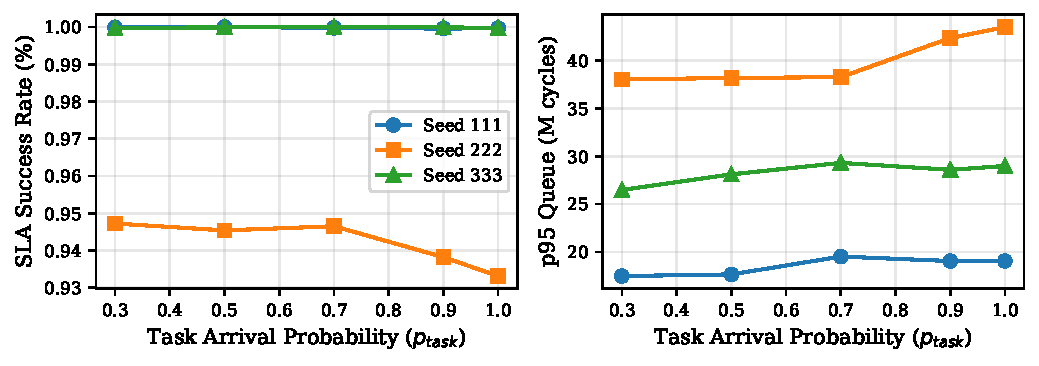
\includegraphics[width=\columnwidth]{figures/fig_matched_outcomes.pdf}
    \caption{Matched congestion outcomes (SLA Success and p95 Queue) across varying task arrival probabilities ($p_{task}$) for the three seeds.}
    \label{fig:matched_outcomes}
\end{figure}

\section{Discussion and Threats to Validity}
\textbf{Practical Implications}: Suppose a production autonomous vehicle company evaluates policies using only average latency or aggregate success rate. They may completely miss latent queue-sensitive representations or fail to detect that their policy's decision boundary lies entirely outside nominal operating conditions. MODE provides the engineering visibility necessary to trust the policy.

\textbf{Threats to Validity}: The primary threat is that the three-seed evaluation reveals substantial seed-dependent instability, but does not provide the statistical power to declare this an inherent FRL law. The observed boundary variability should be interpreted as strong evidence motivating broader stability evaluation across hyper-parameter sweeps and aggregation frequencies. Furthermore, the operational-overlap analysis demonstrates correlation, not causality, between Local execution and SLA preservation.

\section{Conclusion}
The controlled and trajectory-conditioned MODE diagnostics show that the evaluated FedAvg policies develop state-dependent queue sensitivity, but the placement of the learned Local-action region varies substantially across the three training seeds. When this region intersects the empirically reachable joint-state distribution, Local execution is selected during congestion; when it lies outside that distribution, the realized policy remains 5G-dominant despite retaining counterfactual queue sensitivity. These results identify a representation--trajectory mismatch governed jointly by learned decision-surface placement and physical state occupancy. Accordingly, trajectory-level action ratios alone are insufficient to characterize the representational behavior or operational robustness of federated edge policies. 

The proposed diagnostic framework is independent of MA-ROPE~\cite{marope}. Although evaluated on vehicular edge computing, the methodology applies naturally to other safety-critical FRL applications including robotics, autonomous driving, industrial IoT, and distributed edge intelligence. To support further research into representation-aware FRL evaluation, all simulation code, independent and federated training checkpoints, probe scripts, and evaluation environments will be open-sourced as a reproducible benchmark upon publication.

\begin{thebibliography}{00}
\bibitem{marope}
J. Zhao, Y. Sun, Y. Cui, and X. Shen, ``Federated Deep Reinforcement Learning for Resource Allocation in Vehicular Edge Computing,'' \emph{IEEE Transactions on Vehicular Technology}, 2022.
\bibitem{fedavg}
B. McMahan, E. Moore, D. Ramage, S. Hampson, and B. A. y Arcas, ``Communication-Efficient Learning of Deep Networks from Decentralized Data,'' in \emph{AISTATS}, 2017.
\bibitem{dqn}
V. Mnih \emph{et al.}, ``Human-level control through deep reinforcement learning,'' \emph{Nature}, vol. 518, pp. 529--533, 2015.
\end{thebibliography}

\end{document}
